\section{Einführung in die Differentialgleichungen}\label{sec:einfuhrung-in-die-differentialgleichungen}

\subsection{Definition}\label{subsec:definition}

Differentialgleichungen sind eine spezielle Art von \emph{Funktionalgleichungen}: Diese sind Gleichungen, deren Lösungen nicht Zahlen, sondern Funktionen sind.

\begin{definition}{Definition}
    Eine \emph{Differentialgleichung} ist eine Funktionalgleichung, in der (unter anderem) die gesuchte Funktion, ihre Ableitung und ihre Variablen vorkommen.
    Wichtig zu bemerken ist, dass eine Differentialgleichung eine Beziehung zwischen einer Grösse und ihrer Veränderung ausdrückt.
\end{definition}

\textbf{Beispiele:}
\begin{itemize}
    \item $y' = 0$ \\ Eine Lösung: $y = 17$ \\ Allgemeine Lösung: $y = C$ \\ Kontrolle: $y' = (C)' = 0$
    \item $y' = y$ \\ Eine Lösung: $y = e^x$ \\ Allgemeine Lösung: $y = C \cdot e^x$ \\ Kontrolle: $y' = C \cdot e^x = y$
    \item $y' = 7y$ \\ Eine Lösung: $y = e^{7x}$ \\ Allgemeine Lösung: $y = C \cdot e^{7x}$ \\ Kontrolle: $y' = C \cdot 7e^{7x}$, $7y = 7Ce^{7x}$
    \item Beim radioaktiven Zerfall lässt sich die Menge der noch vorhandener Substanz durch folgende Differentialgleichung beschreiben: $y' = -\alpha \cdot y$ ($\alpha$ bezeichnet die sogenannte Proportionalitätskonstante). \\ Eine Lösung: $y = e^{-\alpha t}$ \\ Allgemeine Lösung: $y = C \cdot e^{-\alpha t}$ \\ Kontrolle: $y' = (C \cdot e^{-\alpha t})' = C \cdot (-\alpha) \cdot e^{-\alpha t}$, $-\alpha \cdot y = -\alpha \cdot C \cdot e^{-\alpha t}$
\end{itemize}

\textbf{Bedeutung der Konstanten $C$}

Im obigen Beispiel $t = 0$ einsetzen ergibt $y(0) = C$, d.h. $C$ ist die Menge der Substanz zum Zeitpunkt $t = 0$.
Ist diese Menge $m_0$ vorgegeben, so kommt nur noch eine Lösung infrage: $y(t) = m_0 \cdot e^{-\alpha t}$

Diese Lösung heisst \emph{partikuläre Lösung zur Anfangsbedingung $y(0) = m_0$}, im Gegensatz zur \emph{allgemeinen Lösung}, bei welcher nicht festgelegt ist, welchen Wert die Konstante C annehmen muss.

\begin{definition}{Weitere Definitionen}
    \begin{itemize}
        \item Die \emph{Ordnung} einer Differentialgleichung bezeichnet die Ordnung der höchsten vorkommenden Ableitung.
        \item Die \emph{allgemeine Lösung} einer Differentialgleichung $n$-ter Ordnung ist nie eindeutig bestimmt, sondern enthält noch $n$ voneinander unabhängige Parameter.
        \item Die \emph{partikuläre Lösung} wird durch zusätzliche Bedingungen festgelegt:
        \begin{itemize}
            \item \emph{Anfangsbedingungen:} vorgegebene Werte für $y(x_0)$, $y'(x_0)$, \dots, $y^{(n-1)}(x_0)$
            \item \emph{Randbedingungen:} vorgegebene Werte für $y(x_1)$, $y(x_2)$, \dots, $y(x_n)$
        \end{itemize}
    \end{itemize}
\end{definition}

\newpage

\subsection{Gewöhnliche Differentialgleichungen 1. Ordnung}\label{subsec:gewoehnliche-differentialgleichungen-1.-ordnung}

Eine Differentialgleichung heisst \emph{gewöhnlich}, wenn die gesuchte Funktion eine Funktion von \emph{einer} Variable ist.
Hat die gesuchte Funktion jedoch mehrere Variablen, dann nennt man das eine \emph{partielle} Differentialgleichung.

\begin{definition}{Allgemeine Differentialgleichung 1. Ordnung}
    \emph{Allgemeine Differentialgleichungen 1. Ordnung} haben die Form \[y' = F(x,y)\] wobei $F(x,y)$ ein Ausdruck ist, in dem $x$ und $y$ vorkommen.
\end{definition}

Die \emph{allgemeine} Lösung einer solchen Differentialgleichung enthält einen Parameter, und für jeden Wert dieses Parameters bekommen wir eine Lösung.
Diese Lösungen sind Funktionen und können als Graphen im Koordinatensystem dargestellt werden.

Wir möchten nun Informationen über die Menge dieser Graphen gewinnen.
Dazu fixieren wir einen Punkt $(x_0, y_0)$.
Wenn eine Funktion $f$ eine Lösung der obenstehenden Differentialgleichung ist, dann gilt für jeden Punkt $(x_0, y_0)$ auf ihrem Graph: \[f'(x_0) = F(x_0, y_0)\]
Mit anderen Worten: Falls eine Lösungskurve durch $(x_0, y_0)$ geht, dann hat sie in diesem Punkt die Steigung $F(x_0, y_0)$.
Wir können also diese Steigung ausrechnen, ohne die Lösungsfunktion $f$ zu kennen!

\textbf{Beispiel:} $y' = x-y+1$

Tabelle für $y^{\prime}$ :
\begin{tabular}{|c|c|c|c|c|c|c|c|}
    \hline
    $f'(x_0, y_0)$ & $x_0=-3$ & $x_0=-2$ & $x_0=-1$ & $x_0=0$ & $x_0=1$ & $x_0=2$ & $x_0=3$ \\
    \hline
    $y_0=2$        & -4       & -3       & -2       & -1      & 0       & 1       & 2       \\
    \hline
    $y_0=1$        & -3       & -2       & -1       & 0       & 1       & 2       & 3       \\
    \hline
    $y_0=0$        & -2       & -1       & 0        & 1       & 2       & 3       & 4       \\
    \hline
    $y_0=-1$       & -1       & 0        & 1        & 2       & 3       & 4       & 5       \\
    \hline
    $y_0=-2$       & 0        & 1        & 2        & 3       & 4       & 5       & 6       \\
    \hline
\end{tabular}

\textbf{Skizze des Richtungsfeldes}
\begin{center}
    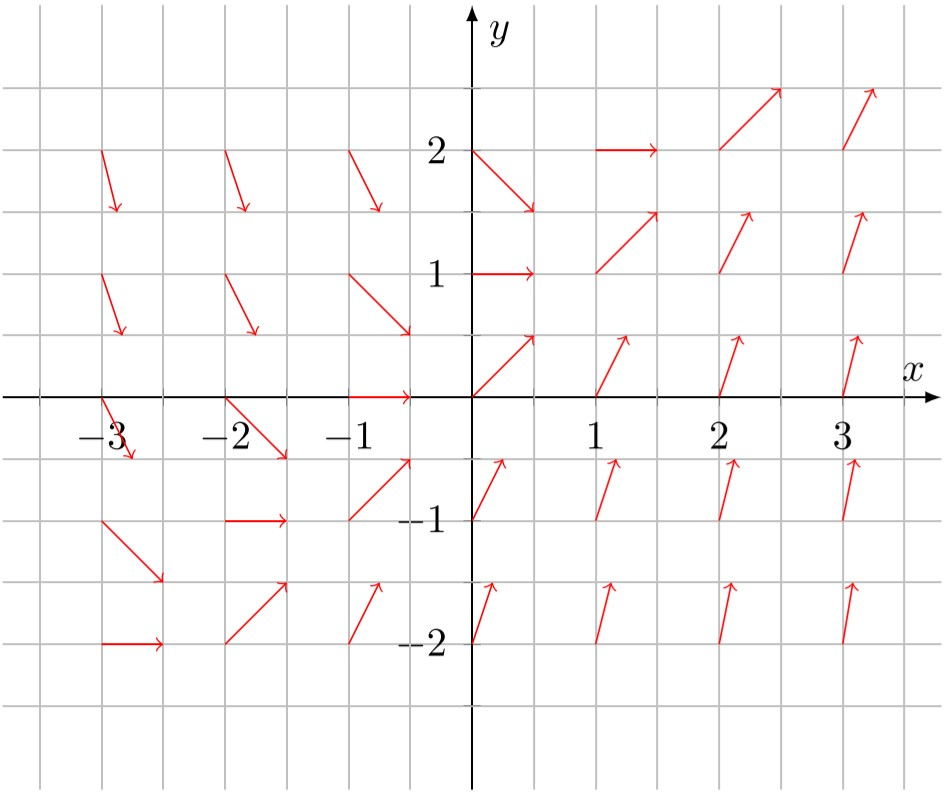
\includegraphics[scale=0.25]{skizze-richtungsfeld}
\end{center}

\textbf{Numerischer Lösungsansatz: Euler-Schritte}

Grund-Idee: An einem Punkt $(x_0,y_0)$ starten und dann der aktuellen Tangente folgen.
\begin{center}
    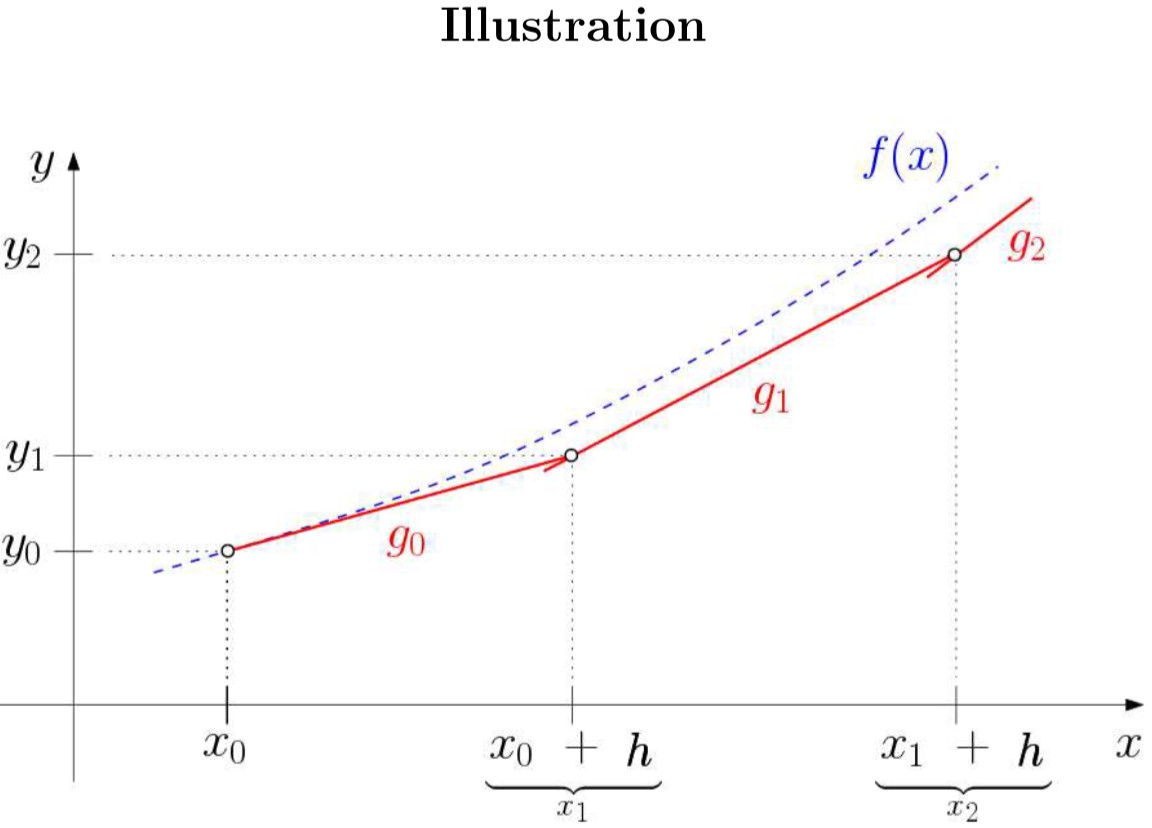
\includegraphics[scale=0.20]{skizze-euler-schritte}
\end{center}

\textbf{Beispiel:} $y' = \underbrace{x+y}_{F(x, y)}$, $x_0 = 0$, $y_0 = 1$, $h = 1$
\begin{center}
    \begin{tabular}{|l|l|l|}
        \hline
        Steigung Gerade &
        Berechnung &
        Beispiel \\
        \hline
        $g_0: m_0=F(x_0, y_0) = x_0 + y_0$   & $x_1 = x_0 + h$                   & $= 0 + 1 = 1$                \\
        & $y_1 = y_0 + h \cdot F(x_0, y_0)$ & $= 1 + 1 \cdot (0 + 1) = 2$  \\
        \hline
        $g_1: m_1 = F(x_1, y_1) = x_1 + y_1$ & $x_2 = x_1 + h$                   & $= 1 + 1 = 2$                \\
        & $y_2 = y_1 + h \cdot F(x_1, y_1)$ & $= 2 + 1 \cdot (1 + 2) = 5$  \\
        \hline
        $g_2: m_2=F(x_2, y_2) = x_2 + y_2$   & $x_3 = x_2 + h$                   & $= 2 + 1 = 3$                \\
        & $y_3 = y_2 + h \cdot F(x_2, y_2)$ & $= 5 + 1 \cdot (2 + 5) = 12$ \\
        \hline
    \end{tabular}
\end{center}

Die obigen Operationen nennt man \emph{Euler-Schritte}.
Der Abstand $h$ zwischen den betrachteten $x$-Werten heisst $Schrittweite$.
Wählt man die Schrittweite sehr, sehr klein, so lassen sich für viele Differentialgleichungen die gewünschten Funktionswerte relativ genau bestimmen.

\subsection{Separierbare Differentialgleichungen}\label{subsec:separierbare-differentialgleichungen}

\begin{definition}{Definition Separierbarkeit}
    Eine Differentialgleichung 1.\ Ordnung heisst \emph{separierbar}, wenn sie sich in der folgenden Form schreiben lässt: \[y' = f(x) \cdot g(y)\]
\end{definition}

\textbf{Beispiele:}
\begin{itemize}
    \item $y' = (x^2 + \sin(x)) \cdot (e^y - y + 7)$ ist eine separierbare Differentialgleichung.
    \item $y' = x - y + 1$ ist \emph{nicht} separierbar.
\end{itemize}

\begin{subbox}{Rezept für die Lösung von separierbaren Differentialgleichungen}
    \begin{enumerate}
        \item $y' = \frac{\diff{y}}{\diff{x}} = f(x) \cdot g(x)$
        \item Trennung der Variablen: $\frac{\diff{y}}{g(y)} = f(x) \cdot \diff{x}$
        \item Integration auf beiden Seiten der Gleichung (falls möglich!) \[\int \frac{\diff{y}}{g(y)} = \int f(x) \diff{x}\]
        \item Auflösen nach $y$ (falls möglich!)
    \end{enumerate}
\end{subbox}

\begin{multicols}{2}
    \textbf{Beispiel 1:} $y' = k \cdot y$
    \begin{enumerate}
        \item $y' = \frac{\diff{y}}{\diff{x}} = k \cdot y$
        \item $\frac{\diff{y}}{y} = k \cdot \diff{x}$
        \item $\int \frac{\diff{y}}{y} = \int k \diff{x} \Rightarrow \ln |y| = k \cdot x + C$
        \item $|y| = e^{kx + C} = e^C \cdot e^{kx} \Rightarrow y = \pm e^C \cdot e^{kx} = \tilde{C} e^{kx}$
    \end{enumerate}

    \textbf{Beispiel 2:} $y' \cdot y^2 = \sin(x)$
    \begin{enumerate}
        \item $y' = \frac{\diff{y}}{\diff{x}} = \frac{\sin(x)}{y^2}$
        \item $y^2 \cdot \diff{y} = \sin(x) \cdot \diff{x}$
        \item $\int y^2 \diff{y} = \int \sin(x) \diff{x} \Rightarrow \frac{1}{3} y^3 = -\cos(x) + C$
        \item $y = (-3\cos(x) + 3C)^{1/3}$
    \end{enumerate}
\end{multicols}

\vspace{-\baselineskip}
\hrulefill

\begin{multicols}{2}
    \textbf{Beispiel 3:} $x + y \cdot y' = 0$ mit Anfangsbedingung $y(3) = -4$
    \begin{enumerate}
        \item $y' = \frac{\diff{y}}{\diff{x}} = - \frac{x}{y}$
        \item $y \cdot \diff{y} = -x \diff{x}$
        \item $\int y \diff{y} = - \int x \diff{x} \Rightarrow \frac{y^2}{2} = - \frac{x^2}{2} + C$
        \item $x^2 + y^2 = C_2$ (Kreisgleichung) \\
        $\Rightarrow y = \pm \sqrt {C_2 - x^2}$ (keine Funktion)
    \end{enumerate}
    \textbf{Einbezug der Anfangsbedingung $y(3) = -4$:}

    Einsetzen von $x = 3, y = -4$ in obige Gleichung liefert:

    $-4 = - \sqrt {C_2 - 9} \Rightarrow C_2 - 9 = 16 \Rightarrow C_2 = 25$

    Lösung: $y = - \sqrt {25 - x^2}$
\end{multicols}

\begin{comment}
    \begin{definition}{Autonome Differentialgleichungen}
        Eine Differentialgleichung heisst \emph{autonom}, wenn sie sich in der folgenden Form darstellen lässt: \[y' = f(y)\]
    \end{definition}

    \textbf{Beispiele}
    \begin{center}
        \begin{tabular}{|l|l|}
            \hline
            \multicolumn{1}{|c|}{ Gleichung }            & Autonom?                                                      \\
            \hline
            $y' = y^2 + 6$                               & Ja $\Rightarrow f(y) = y^2 + 6$                               \\
            \hline
            $y' = x + y$                                 & Nein                                                          \\
            \hline
            $y' = \frac{y}{x}$                           & Nein                                                          \\
            \hline
            $y' = y^2 \cdot \sqrt{1 - \sin(y)} - \ln(y)$ & Ja $\Rightarrow f(y) = y^2 \cdot \sqrt{1 - \sin(y)} - \ln(y)$ \\
            \hline
        \end{tabular}
    \end{center}

    \textbf{Lösungsmethode:} Diese Differentialgleichungen sind separierbar!
\end{comment}

\subsection{Lineare Differentialgleichungen 1. Ordnung}\label{subsec:lineare-differentialgleichungen-1.-ordnung}

\begin{definition}{Lineare Differentialgleichungen}
    Eine Differentialgleichung 1.\ Ordnung heisst \emph{linear}, wenn sie die Form \[y' + f(x) \cdot y = g(x)\] hat, wobei $f$ und $g$ Funktionen von $x$ sind.
    Die Funktion $g(x)$ wird als \emph{Störglied} oder \emph{Störfunktion} bezeichnet.
\end{definition}

\textbf{Bemerkung:} Die Bezeichnung \emph{linear} bezieht sich einzig darauf, dass $y$ und $y'$ nur in der ersten Potenz vorkommen.
Die Funktionen $f(x)$ und $g(x)$ hingegen brauchen keineswegs linear zu sein.

\begin{center}
    \begin{tabular}{|c|c|c|}
        \hline
        Differentialgleichung                                    & $f(x)$        & $g(x)$                          \\
        \hline
        $y' = xy$                                                & $-x$          & $0$                             \\
        \hline
        $xy' + 2y = e^x$                                         & $\frac{2}{x}$ & $\frac{e^x}{x}$                 \\
        \hline
        $y' = (\tan(x)) \cdot y + 2 \cdot \sin(x) \cdot \cos(x)$ & $-\tan(x)$    & $2 \cdot \sin(x) \cdot \cos(x)$ \\
        \hline
    \end{tabular}
\end{center}

\begin{definition}{Homogene DGL}
    Eine lineare Differentialgleichung heisst \emph{homogen}, wenn das Störglied $g(x) = 0$ ist.
    Ansonsten nennt man sie \emph{inhomogen}.

    Betrachtet man eine \emph{inhomogene} lineare Differentialgleichung $y' + f(x) \cdot y = g(x)$, dann bezeichnet man die \emph{zugehörige homogene Differentialgleichung} die Gleichung $y_0' + f(x) \cdot y_0 = 0$.
\end{definition}

Grundsätzlich sind homogene Differentialgleichungen leichter zu lösen als inhomogene.
Unser Lösungsverfahren für lineare Differentialgleichungen besteht deshalb aus zwei Schritten:
\begin{enumerate}
    \item Lösung der zugehörigen Differentialgleichung bestimmen.
    \item Ursprüngliche Differentialgleichung durch \emph{Variation der Konstanten} lösen.
\end{enumerate}

\begin{subbox}{Rezept: Variation der Konstanten}
    \begin{enumerate}
        \item Vergleich der \emph{gegebenen} Differentialgleichung mit der \emph{allgemeinen} Form $y' + f(x) \cdot y = g(x)$ und Bestimmung von $f(x)$ und $g(x)$.
        \item Bestimmung der Stammfunktion $F(X)$ von $f(x)$.
        \item Einsetzen in die Formel $y_0 = C \cdot e^{-F(x)}$ liefert die Lösung der zugehörigen \emph{homogenen} Differentialgleichung.
        \item Ein Einsetzen von $C$ durch eine noch zu bestimmende Funktion $K(x)$ führt zum folgenden Ansatz für die allgemeine Lösung: \[y = K(x) \cdot e^{-F(x)}\]
        \item Die Funktion $K(x)$ lässt sich durch die folgende Formel berechnen: \[K(x) = \int g(x) \cdot e^{F(x)} \diff{x} \quad\quad\quad \text{(Integrationskonstante nicht vergessen!)}\]
        \item Einsetzen von $K(x)$ in den Ansatz aus Schritt 4 ergibt die \emph{allgemeine Lösung}.
    \end{enumerate}
\end{subbox}

\textbf{Beispiel:} $y' + \frac{y}{x} = \cos(x)$
\begin{enumerate}
    \item $f(x) = \frac{1}{x}$, $g(x) = \cos(x)$
    \item $F(x) = \ln(x)$
    \item $y_0 = \frac{C}{x}$
    \item Ansatz: $y = \frac{K(x)}{x}$
    \item $K(x) = \int g(x) \cdot e^{F(x)} \diff{x} = \int \cos(x) \cdot x \diff{x} = x \cdot \sin(x) + \cos(x) + C_2$
    \item $K(x)$ in den Ansatz von Schritt 4 einsetzen: $y = \frac{x \cdot \sin(x) + \cos(x) + C_2}{x}$
\end{enumerate}